\documentclass{beamer}
\setbeamertemplate{navigation symbols}{}
\usepackage{comment}

\setbeamercolor{frametitle}{fg=black,bg=white}
\setbeamercolor{title}{fg=black,bg=yellow!85!orange}
\usetheme{AnnArbor}

\usepackage{textpos} % package for the positioning
\usepackage{listings}
\usepackage{xcolor}
\usepackage[most]{tcolorbox}
\usepackage{mathtools}
\usepackage{graphicx}
\usepackage{graphbox}
\usepackage{caption}
\DeclareCaptionType{code}[Code Listing][List of Code Listings] 

\definecolor{codegreen}{rgb}{0,0.6,0}
\definecolor{codegray}{rgb}{0.5,0.5,0.5}
\definecolor{codepurple}{rgb}{0.58,0,0.82}
\definecolor{backcolour}{rgb}{0.95,0.95,0.92} 
\lstdefinestyle{mystyle}{
    backgroundcolor=\color{backcolour},   
    commentstyle=\color{codegreen},
    keywordstyle=\color{magenta},
    numberstyle=\tiny\color{codegray},
    stringstyle=\color{codepurple},
    basicstyle=\ttfamily\footnotesize,
    breakatwhitespace=false,         
    breaklines=true,                 
    captionpos=b,                    
    keepspaces=true,                 
    numbers=left,                    
    numbersep=5pt,                  
    showspaces=false,                
    showstringspaces=false,
    showtabs=false,                  
    tabsize=2
}

\lstset{style=mystyle}

\lstdefinelanguage
   [x64]{Assembler}     % add a "x64" dialect of Assembler
   [x86masm]{Assembler} % based on the "x86masm" dialect
   % with these extra keywords:
   {morekeywords={CDQE,CQO,CMPSQ,CMPXCHG16B,JRCXZ,LODSQ,MOVSXD, %
                  POPFQ,PUSHFQ,SCASQ,STOSQ,IRETQ,RDTSCP,SWAPGS, %
                  rax,rdx,rcx,rbx,rsi,rdi,rsp,rbp, %
                  r8,r8d,r8w,r8b,r9,r9d,r9w,r9b, %
                  r10,r10d,r10w,r10b,r11,r11d,r11w,r11b, %
                  r12,r12d,r12w,r12b,r13,r13d,r13w,r13b, %
                  r14,r14d,r14w,r14b,r15,r15d,r15w,r15b}} %


\beamersetuncovermixins{\opaqueness<1>{25}}{\opaqueness<2->{15}}

%Copyright
\addtobeamertemplate{frametitle}{}{%
\begin{textblock*}{50mm}(0cm,-1.25cm)
\color{yellow!85!orange}
\tiny{Copyright \copyright 2024 CNM.}
\end{textblock*}}

% position the logo
\addtobeamertemplate{frametitle}{}{%
\begin{textblock*}{100mm}(11.4cm,-1.3cm)

\includegraphics[height=1cm,width=1cm,keepaspectratio]{fig/ddclogotransparent.png}
\end{textblock*}}

\AtBeginSection[]{
  \begin{frame}
  \vfill
  \centering
  \begin{beamercolorbox}[sep=8pt,center,shadow=true,rounded=true]{title}
    \usebeamerfont{title}\insertsectionhead\par%
  \end{beamercolorbox}
  \vfill
  \end{frame}
}

\begin{document}
\title{Quantum Math}
\author{Brian Rashap}
\date{August 2025} 



\begin{frame}
\titlepage
\end{frame}

\section{Algebra}
\begin{frame}\frametitle{Algebra Overview}
\begin{itemize}
\item Functions
\item Transformations
\item Polynomials
\item Rational Functions
\item Exponentials and Logarithms
\end{itemize}
\end{frame}

\begin{frame}\frametitle{Cartesian Coordinates}
\begin{columns}
\begin{column}{4cm}
Some text
\end{column}
\begin{column}{6cm}
\begin{center}
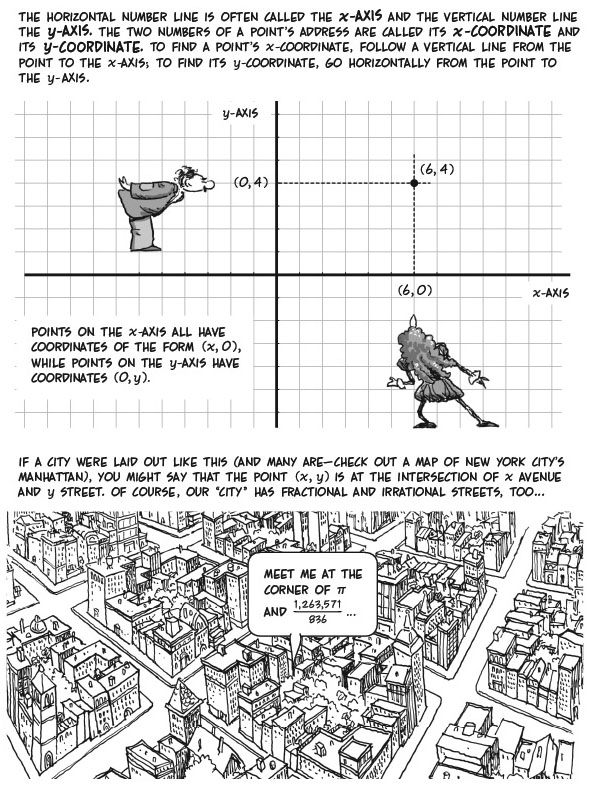
\includegraphics[height=7.5cm]{fig/plotting.jpg}
\end{center}
\end{column}
\end{columns}
\end{frame}

\begin{frame}\frametitle{Measuring Distance - Pythagorean Theorem}
\begin{columns}
\begin{column}{6cm}
Pythagorean Theorem:
\begin{center}
$a^2 + b^2 = c^2$
\end{center}

For example: \newline

\hspace*{10mm}$d^2 = 3^2 + 4^2$ \newline
\hspace*{10mm}$d^2 = 9 + 16 = 25$ \newline
\hspace*{10mm}$d = \sqrt{25} = 5$ \newline

More generally for two points $P(x_1,y_1)$ and $Q(x_2,y_2)$ \newline

\hspace*{10mm}$d^2 = (x_2-x_1)^2 + (y_2 - y_1)^2$ \newline
\hspace*{10mm}$d = \sqrt{(x_2-x_1)^2 + (y_2 - y_1)^2}$ \newline

Noting that $\mid a \mid = (a)^2$: \newline


\end{column}
\begin{column}{5cm}
\begin{center}
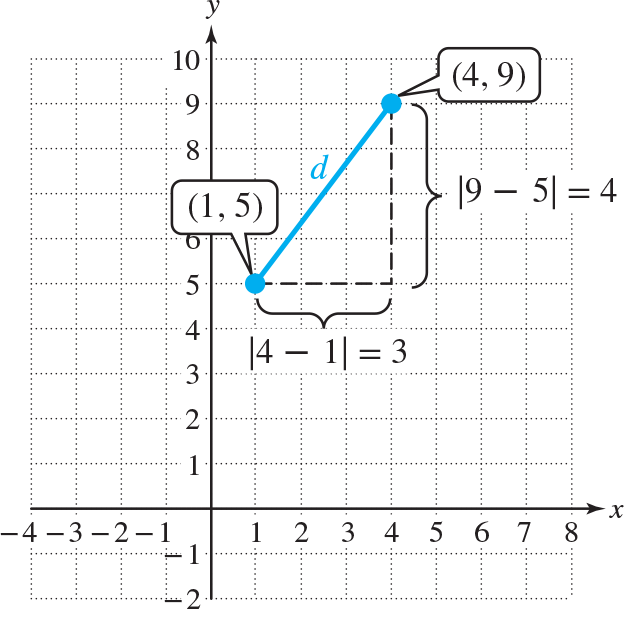
\includegraphics[width=4cm]{fig/pythag.png}
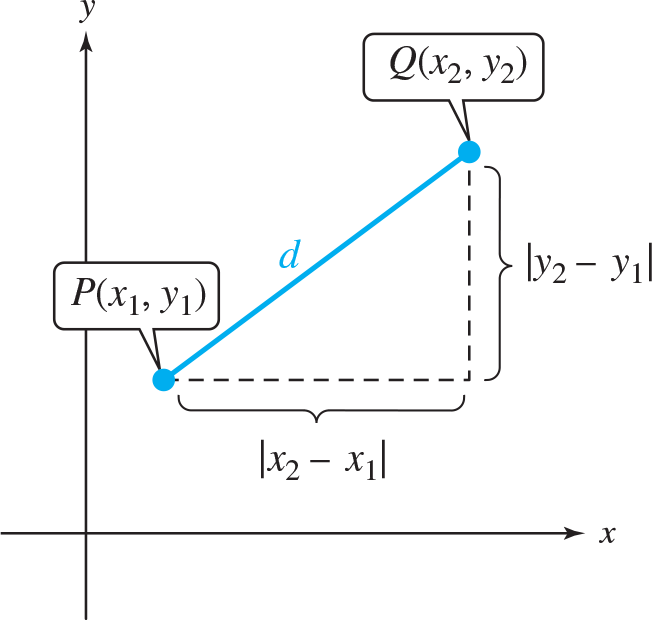
\includegraphics[width=4cm]{fig/pythag2.png}
\end{center}
\end{column}
\end{columns}
\end{frame}

\begin{frame}\frametitle{Midpoints and Intercepts}
\begin{columns}
\begin{column}{6cm}

Midpoint: \newline

\hspace*{10mm}$M = (\frac{x_1+x_2}{2},\frac{y_2+y_1}{2})$ \newline


Intercepts: \newline

Two key features of a graph are where the graph intersects the x and y axes, the x-intercept and y-intercept, respectively.


\end{column}
\begin{column}{5cm}
\begin{center}
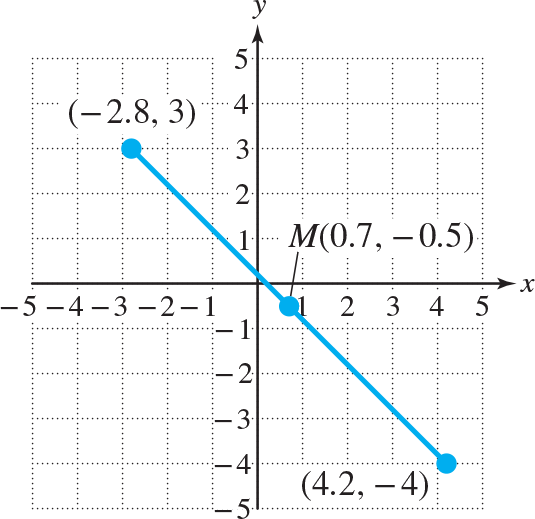
\includegraphics[width=4cm]{fig/midpoint.png}
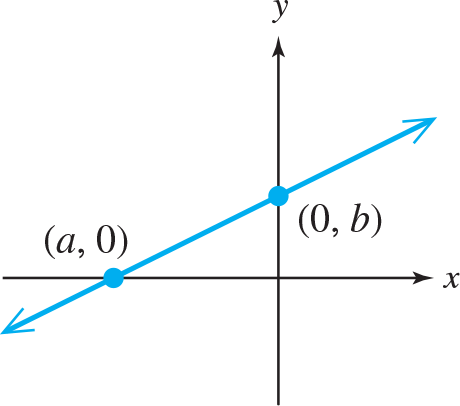
\includegraphics[width=4cm]{fig/intercept.png}
\end{center}
\end{column}
\end{columns}
\end{frame}


\begin{frame}\frametitle{The Circle}
\begin{columns}
\begin{column}{7.5cm}

A circle is a set of all points that are equidistant from a fixed point called the center $(h,k)$. The distance from any point on the cirecle to the center is called the radius ($r$)

$r = \sqrt{(x-h)^2 + (y-k)^2}$ \newline

Equation of a circle: \newline
Standard form: $(x-h)^2 + (y-k)^2 = r^2$ \newline

Expand binomials: $x^2-hx+h^2+y^2-ky+k^2 - r^2 = 0$ \newline

General form: $x^2+y^2-hx-ky+(h^2+k^2-r^2)=0$

\hspace*{10mm} or

$x^2 + y^2 + Ax + By + C = 0$

\end{column}
\begin{column}{3.5cm}
\begin{center}
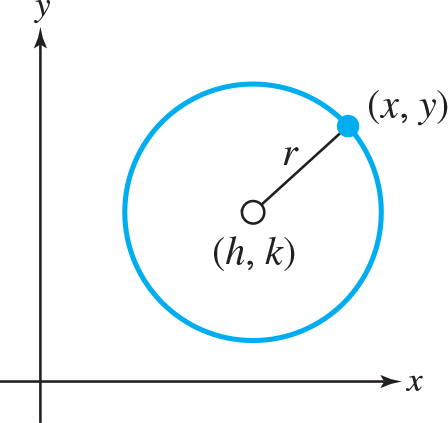
\includegraphics[width=3cm]{fig/circle.png}
\end{center}
\end{column}
\end{columns}
\end{frame}



\begin{frame}\frametitle{Domain and Range}
\begin{columns}
\begin{column}{6cm}
\begin{center}
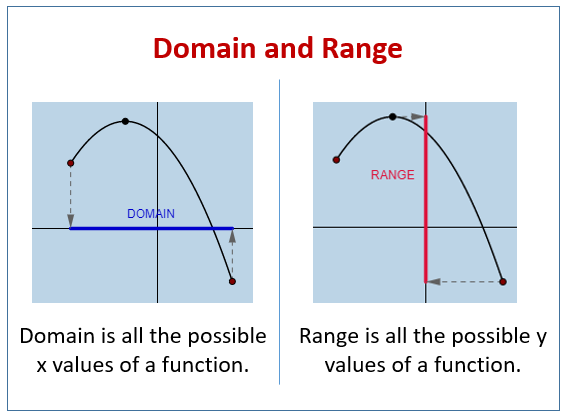
\includegraphics[width=6cm]{fig/domain-range.png}
\end{center}
\end{column}

\begin{column}{5cm}
A set of ordered pairs $(x,y)$ is called a relation in x and y. 
\begin{itemize}
\item The set of x-values in the ordered pairs is called the domain of the relations.
\item The set of y-values in the ordered pairs is called the range of the relations.
\end{itemize}
\end{column}
\end{columns}
\end{frame}


\begin{frame}\frametitle{Linear Equations with Two Variables}
A linear equation in variables $x$ and $y$ can be written in the standard form:
\begin{equation}
Ax + By = C
\end{equation}

However, it is more common to see it in slope-intercept form:
\begin{equation}
y = mx + b
\end{equation}
where, $m$ is the slope and $b$ is the y-intercept
\end{frame}

\begin{frame}\frametitle{Linear Conversion - Slope and Y-Intercept}
\begin{columns}
\begin{column}{6cm}
\begin{center}
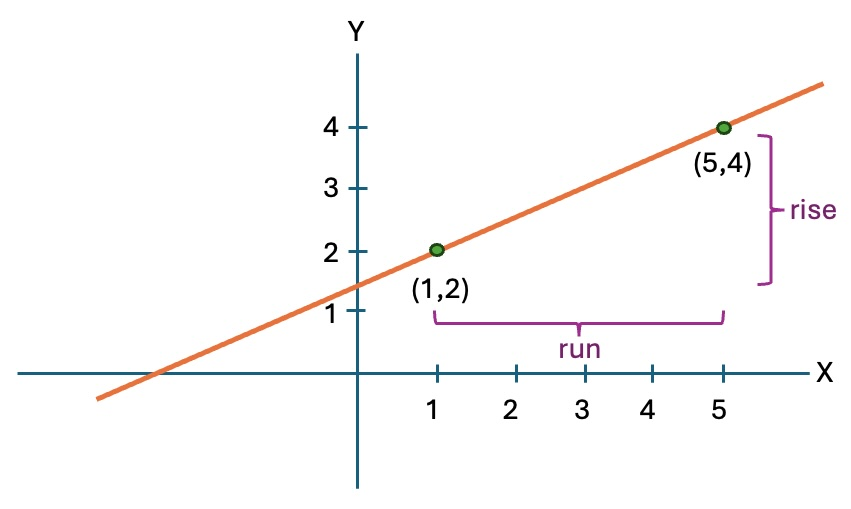
\includegraphics[width=5cm]{fig/slope.jpg}

$y = mx + b$

where $m$ is slope and $b$ y-intercept. 
\end{center}
\end{column}

\begin{column}{5.2cm}
For example, given two points:
\begin{itemize}
\item $(x_1,y_1) = (1,2)$
\item $(x_2,y_2) = (5,4)$
\end{itemize}
Find slope
\begin{itemize}
\item $m = \frac{rise}{run} = \frac{4-2}{5-1} = \frac{1}{2}$
\end{itemize}
Find y-intercept
\begin{itemize}
\item $y_1 = m * x_1 + b$
\item $b = y_1 - (m * x_1$)
\item $b = 2 - (\frac{1}{2} * 1) = 1 \frac{1}{2}$
\end{itemize}
\end{column}
\end{columns}

\vspace{1cm}

Use this to find the conversion from Celsius to Fahrenheit.
\end{frame}

\begin{frame}\frametitle{Parallel and Perpendicular Lines}
\begin{center}
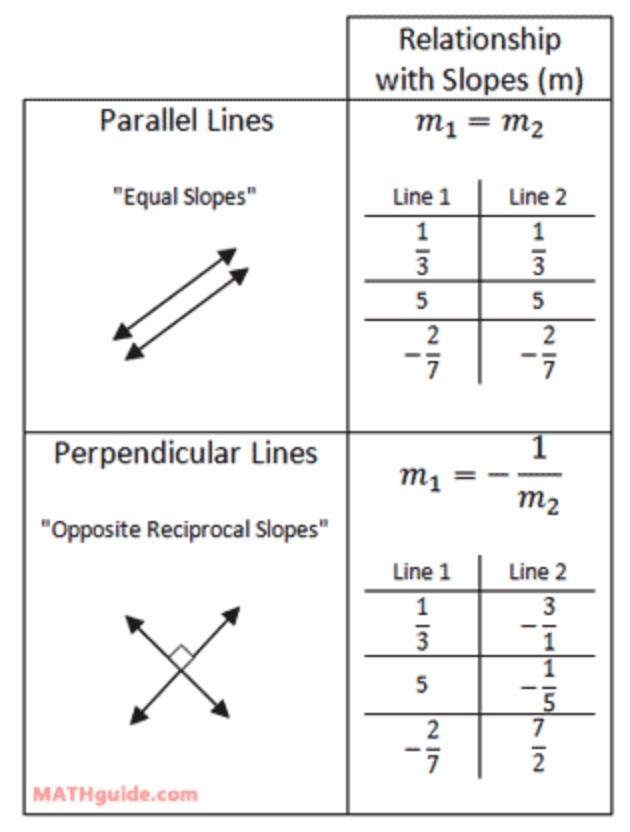
\includegraphics[width=5.5cm]{fig/parperp.jpg}
\end{center}
\end{frame}



\begin{frame}\frametitle{Linear Regression}
\begin{columns}
\begin{column}{6cm}
\begin{center}
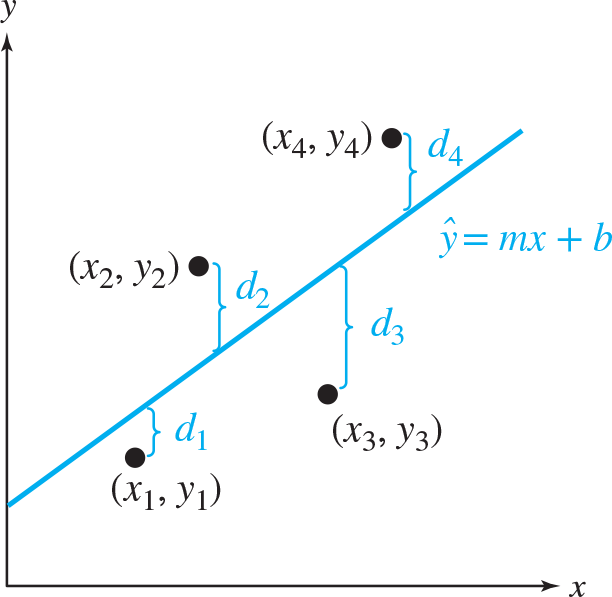
\includegraphics[width=5cm]{fig/lsqr.png}
\end{center}
\end{column}

\begin{column}{5cm}
Consider a set of data: $(x_1,y_1),(x_2,y_2),(x_3,y_3),...,(x_n,y_n)$
\begin{itemize}
\item The least-squares regression line $\hat{y} = mx + b$, is a unique line that minimizes the sum of the squared vertical deviations from the the observed data points to the line.
\end{itemize}
\end{column}
\end{columns}

\vspace{1cm}

Use this to find the conversion from Celsius to Fahrenheit.
\end{frame}


\begin{frame}\frametitle{Recognizing Functions}
\begin{columns}
\begin{column}{4.5cm}
An algebraic function provides a "y-value" for every "x-value"
\begin{itemize}
\item Linear: $y = x + 2$
\item Quadratic: $y = x^2$
\item Periodic: $y = sin(x)$
\end{itemize}
\end{column}
\begin{column}{7cm}
\begin{center}
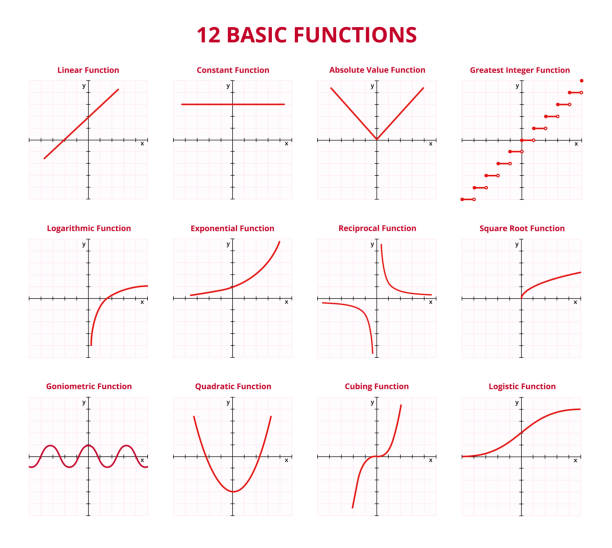
\includegraphics[width=7cm]{fig/basicfun.jpg}
\end{center}
\end{column}
\end{columns}
\end{frame}


\begin{frame}\frametitle{Vertical and Horizontal Shifts}
\begin{columns}
\begin{column}{5.0cm}
\begin{center}
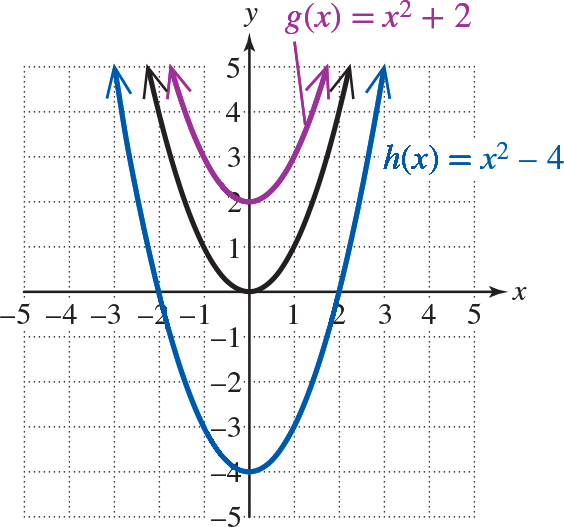
\includegraphics[height=4.5cm]{fig/shiftV.png}
\end{center}
\end{column}
\begin{column}{6.0cm}
\begin{center}
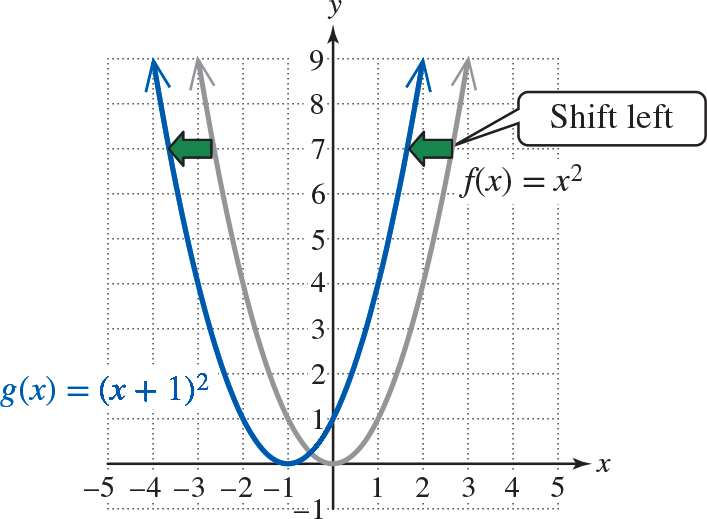
\includegraphics[height=4.5cm]{fig/shiftH.png}
\end{center}
\end{column}
\end{columns}
\end{frame}

\begin{frame}\frametitle{Shrink and Expand}

\begin{center}
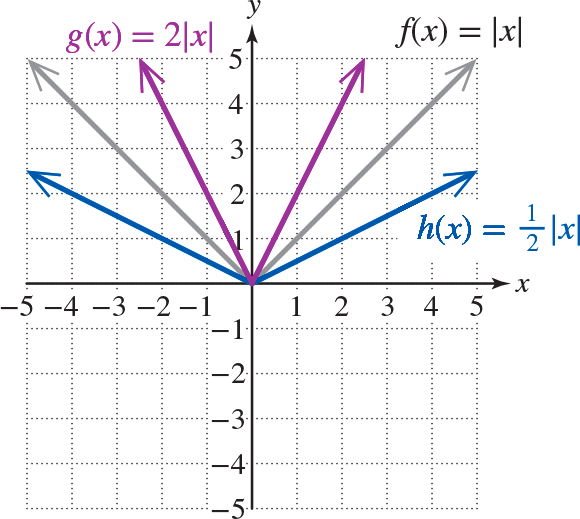
\includegraphics[height=6.0cm]{fig/stretchV.png}
\end{center}

\end{frame}


\begin{frame}\frametitle{X and Y Reflections}
\begin{columns}
\begin{column}{5.5cm}
\begin{center}
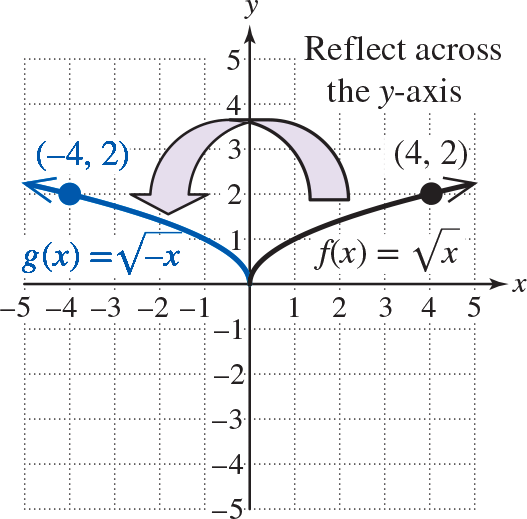
\includegraphics[height=4.5cm]{fig/reflectX.png}
\end{center}
\end{column}
\begin{column}{5.5cm}
\begin{center}
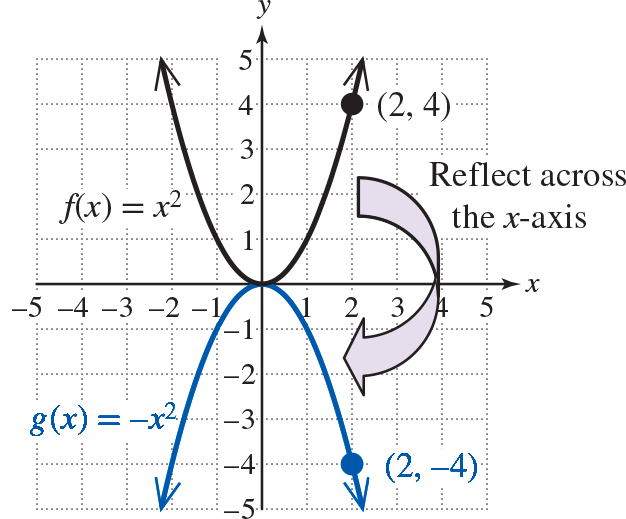
\includegraphics[height=4.5cm]{fig/reflectY.png}
\end{center}
\end{column}
\end{columns}
\end{frame}

\begin{frame}\frametitle{Summary - Transformations of Functions}
\begin{center}
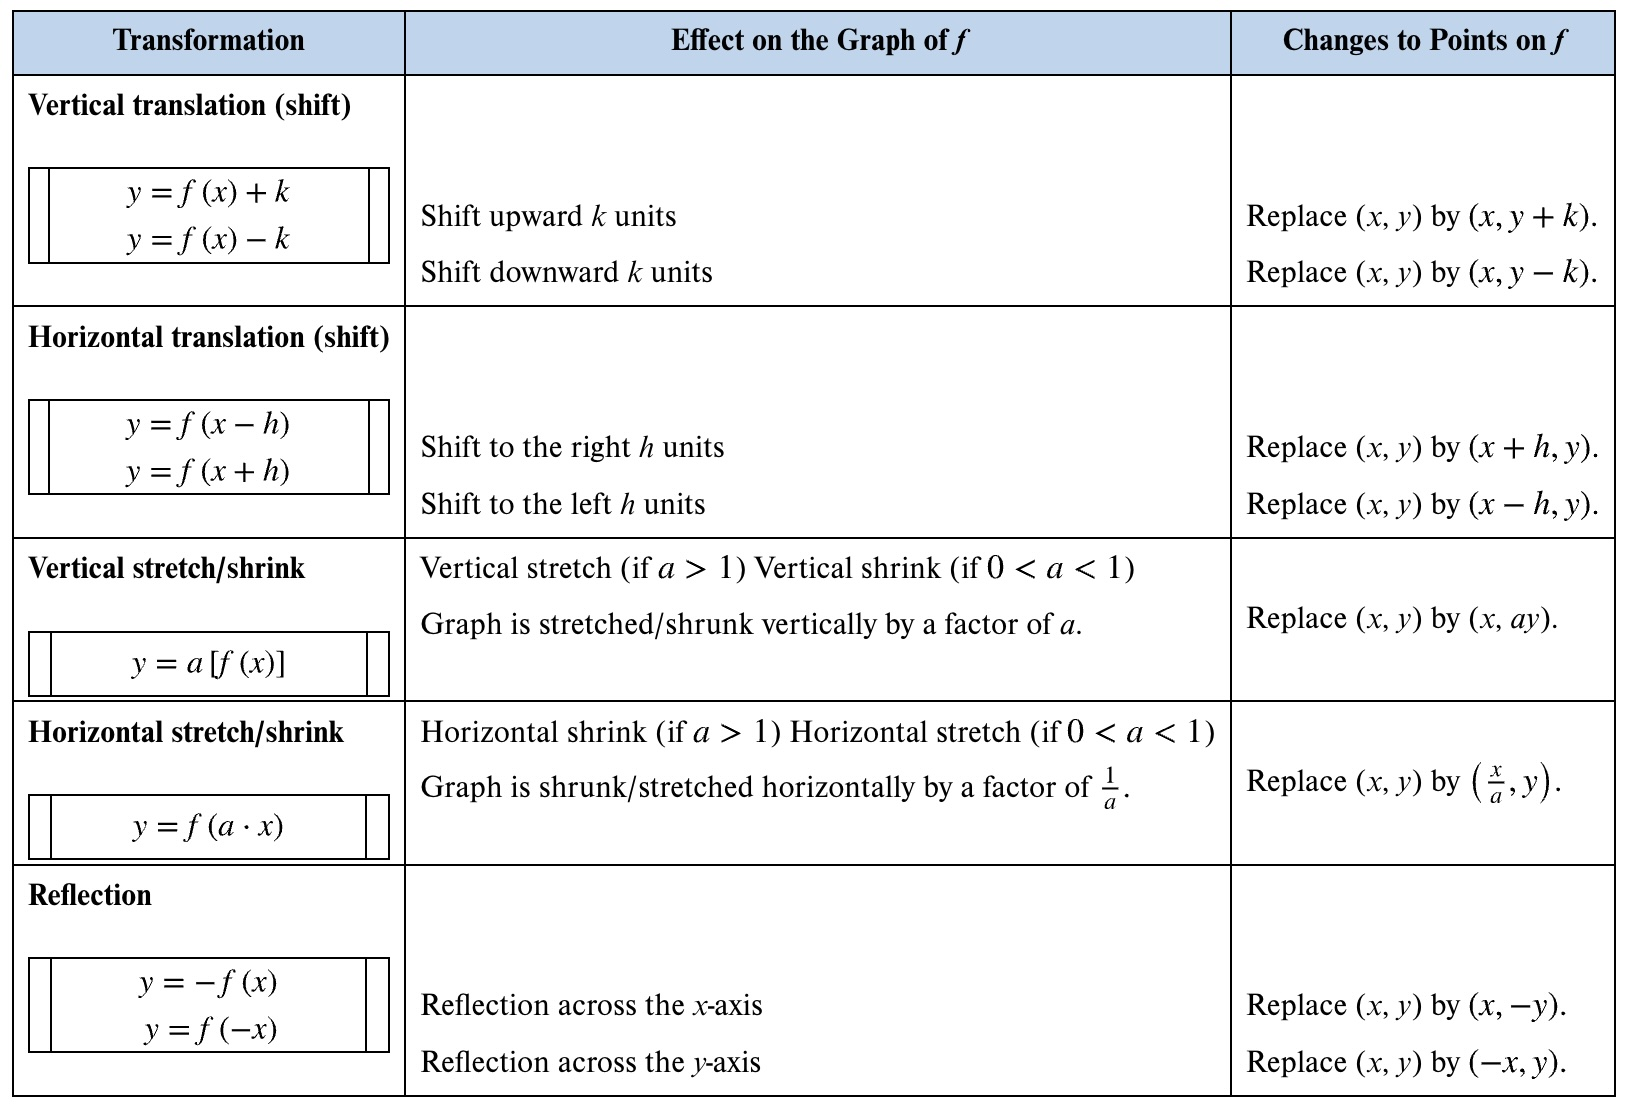
\includegraphics[width=10cm]{fig/transform.jpg}
\end{center}
\end{frame}


\begin{frame}\frametitle{Piece-Wise Functions}
\begin{columns}
\begin{column}{6cm}
\begin{center}
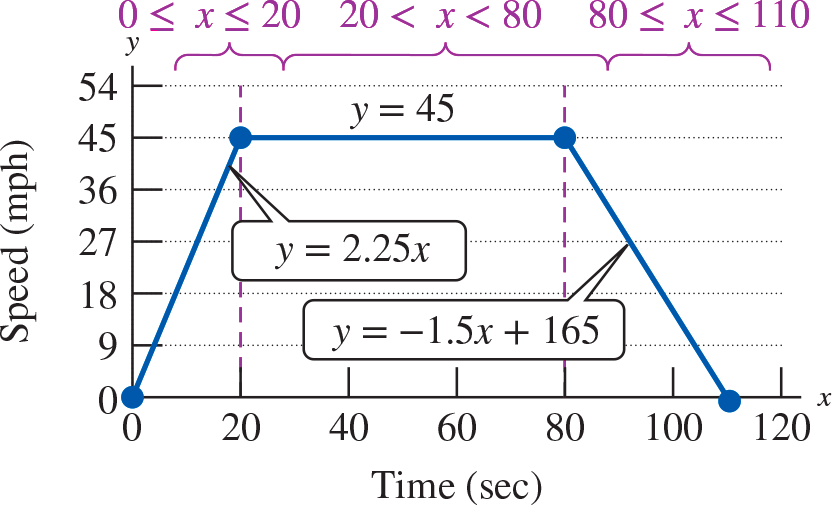
\includegraphics[width=6cm]{fig/pwfunct1.png}
\end{center}
\end{column}
\begin{column}{5cm}
\begin{center}
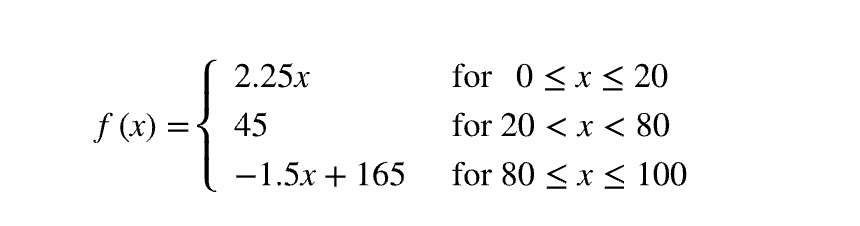
\includegraphics[width=6cm]{fig/pwfunct2.jpg}
\end{center}
\end{column}
\end{columns}
\end{frame}

\begin{frame}\frametitle{Rate of Change}

\end{frame}

\begin{frame}\frametitle{Operations on Functions}

\end{frame}


\begin{frame}\frametitle{Exponential Functions}
\begin{itemize}
\item Linear growth - a constant rate of change, that is,a constant number by which the output increased for each unit increase in input.
\item Exponential growth - increase based on a constant multiplicative rate of change over equal increments of time, that is, a percent increase of the original amount over time.
\end{itemize}

\begin{center}
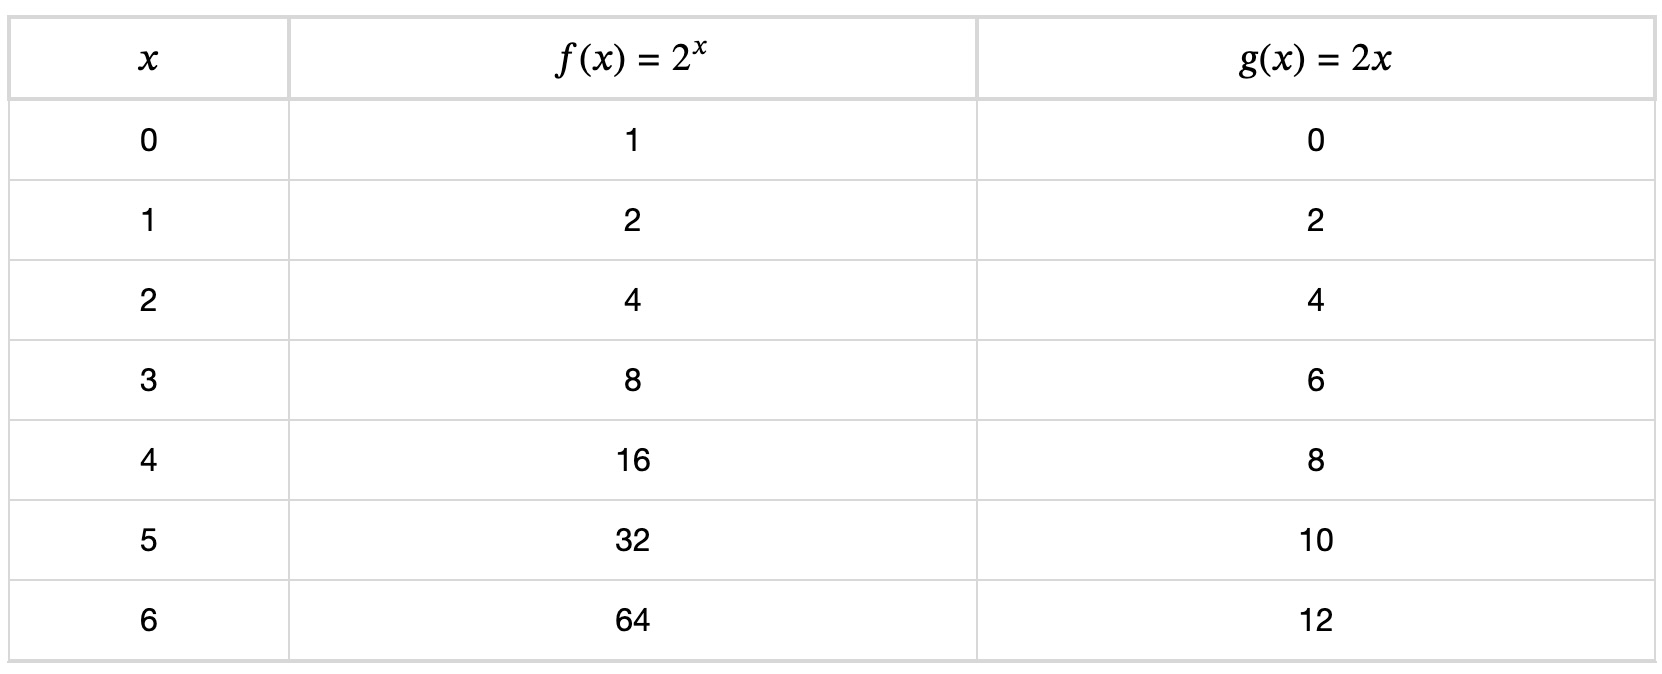
\includegraphics[width=12cm]{fig/exp_growth.jpg}
\end{center}

\end{frame}


\begin{frame}\frametitle{Origami to the Moon}
\begin{center}
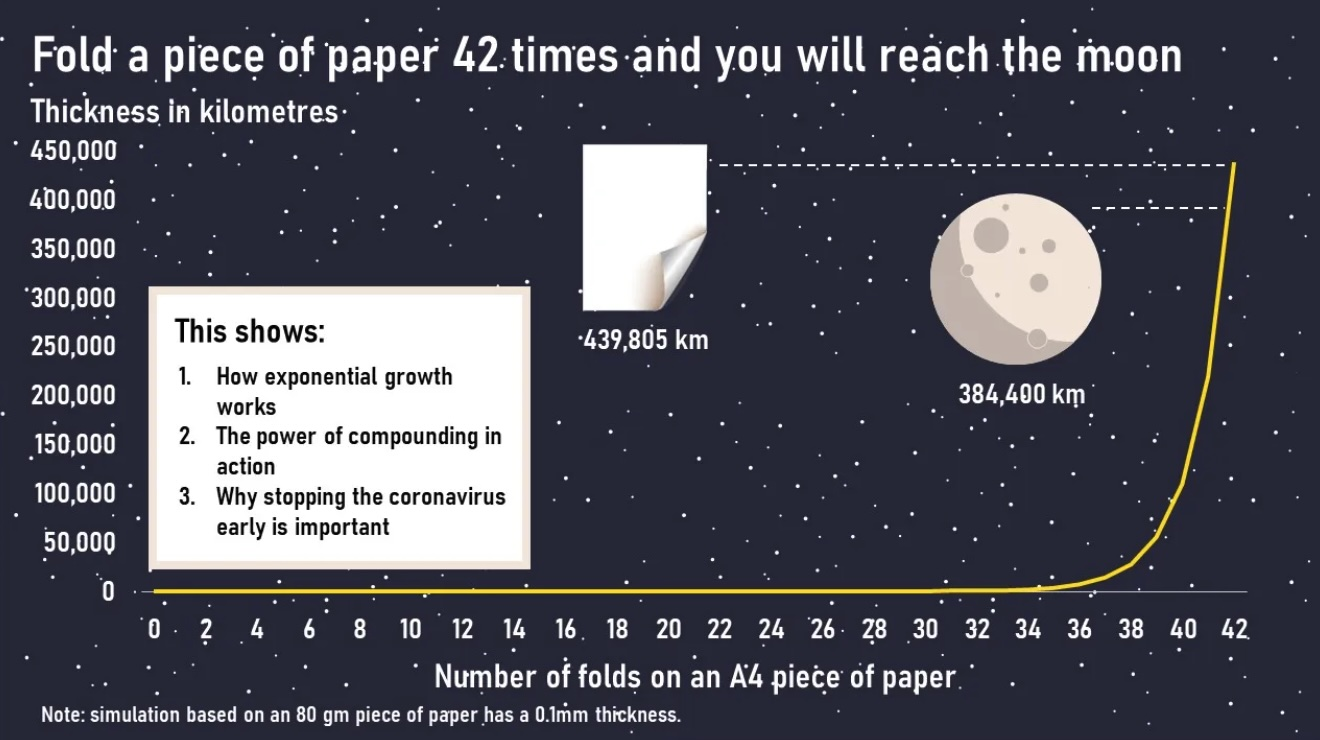
\includegraphics[width=12cm]{fig/40fold.jpg}
\end{center}
\end{frame}

\begin{frame}\frametitle{What about Negative Exponents}
\begin{columns}
\begin{column}{7cm}
The general form of an exponential function is $f(x) = ab^x$, where $a$ is any non-zero number and $b$ is an positive number not equal to 1.

\begin{itemize}
\item If $b > 1$ the function grows at a rate proportional to its size.
\item If $0 < b < 1$ the function decays at a rate proportional to its size.
\end{itemize}
\end{column}

\begin{column}{5cm}
For example, $f(x) = 2^x$:
\begin{center}
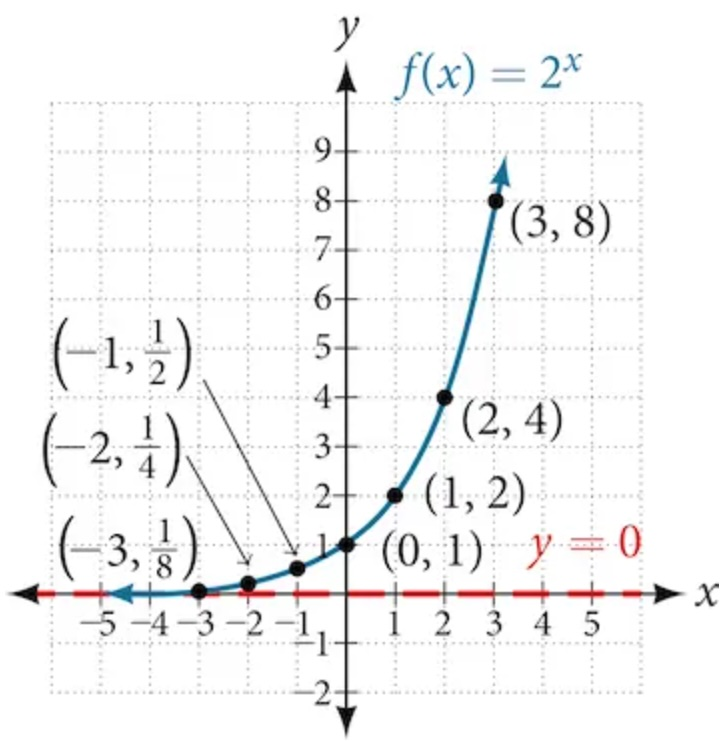
\includegraphics[width=4cm]{fig/exp2g.jpg}
\end{center}
\end{column}
\end{columns}

\begin{center}
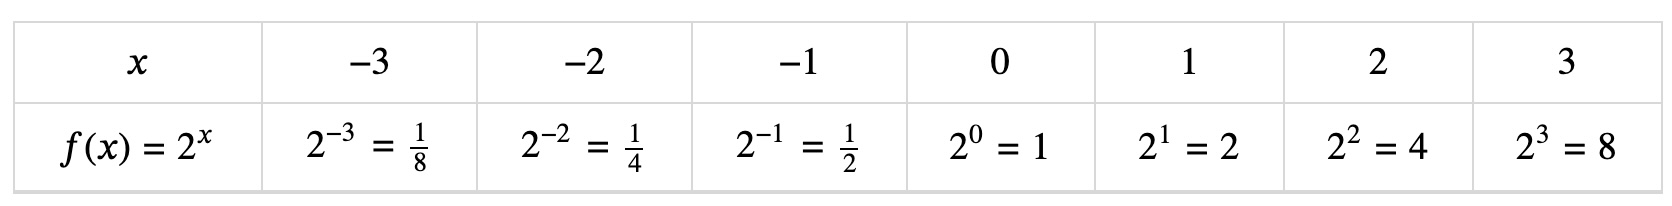
\includegraphics[width=12cm]{fig/exp2t.jpg}
\end{center}
\end{frame}

\begin{frame}\frametitle{Scientific (SI) Prefixes}
\begin{center}
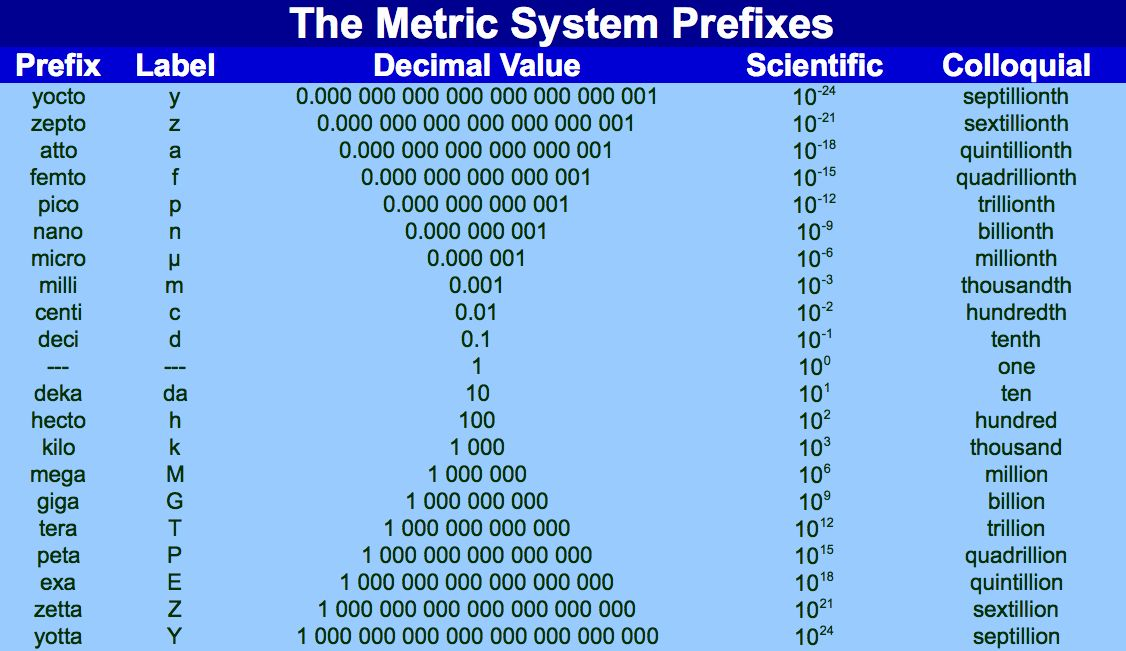
\includegraphics[width=12cm]{fig/si_prefixes.jpg}
\end{center}
\end{frame}

\begin{frame}\frametitle{$e$ - an interesting aside}
The letter e represents the irrational number:
\begin{equation}
e = (1 + \frac{1}{n})^n
\end{equation}
as $n$ increases without bound. \newline



The number $e$ is used as a base for many real-world exponential models. To work with base e, we use the approximation,  $e \approx 2.718282$. The constant was named by the Swiss mathematician Leonhard Euler (1707–1783) who first investigated and discovered many of its properties.
\end{frame}


\begin{frame}\frametitle{Graphing Exponentials}
\begin{columns}
\begin{column}{7cm}

Shifts:
\begin{center}
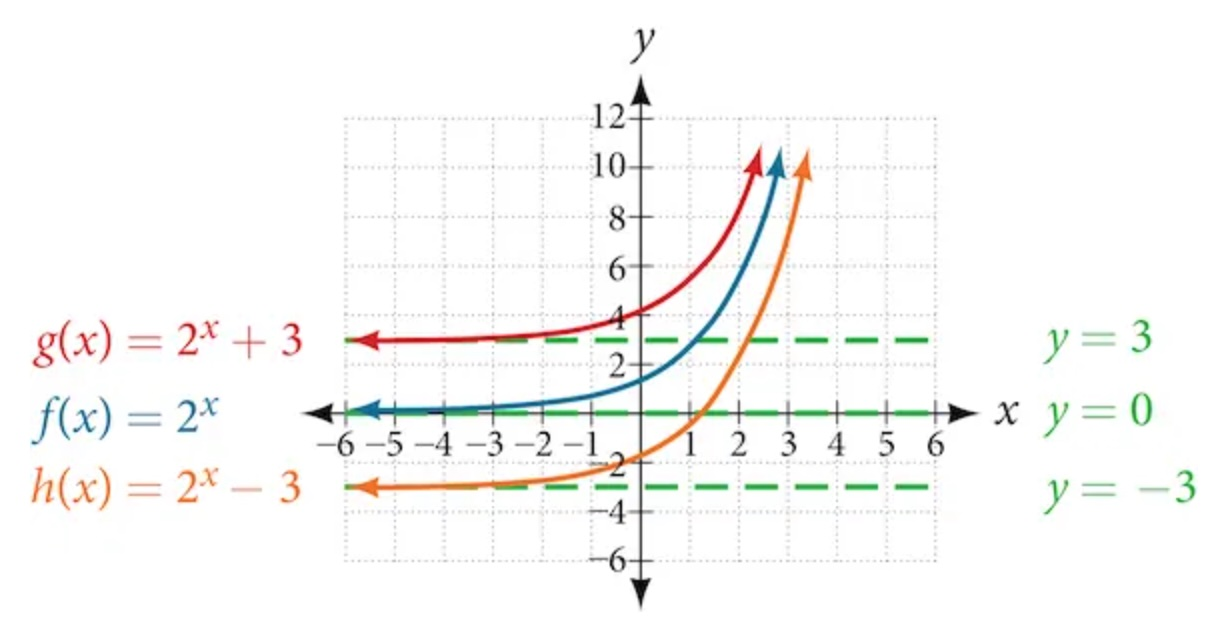
\includegraphics[width=6.5cm]{fig/exp2vert.jpg}
\end{center}

\begin{center}
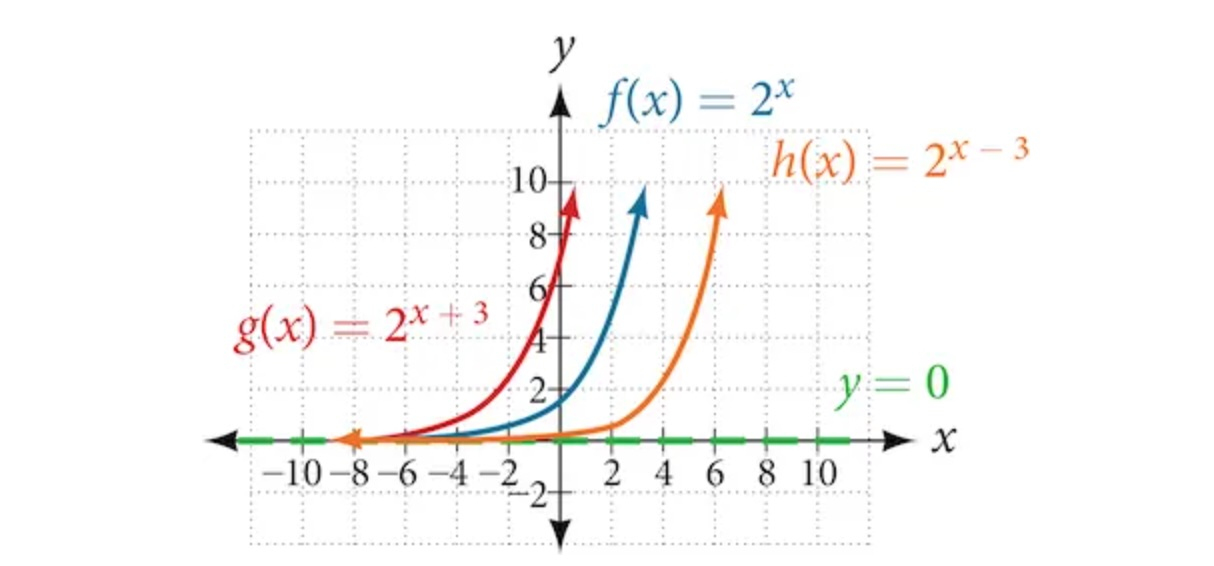
\includegraphics[width=6.5cm]{fig/exp2hor.jpg}
\end{center}

\end{column}

\begin{column}{5cm}
Stretch:
\begin{center}
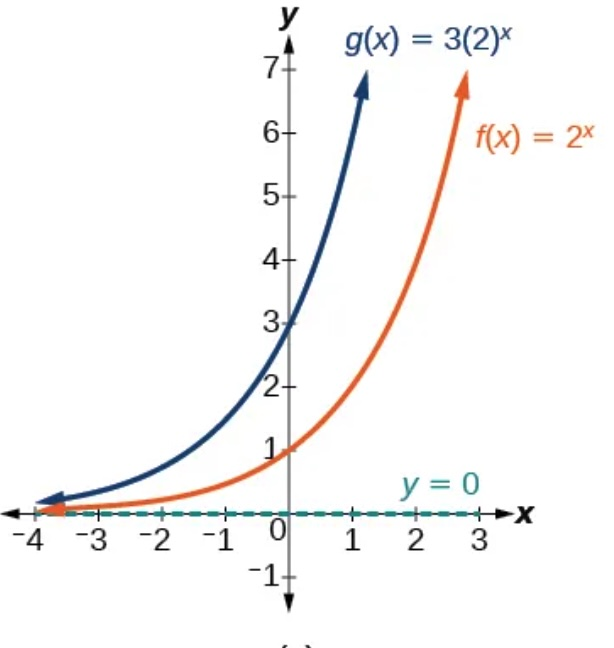
\includegraphics[width=2.8cm]{fig/exp2v.jpg}
\end{center}

Flip:
\begin{center}
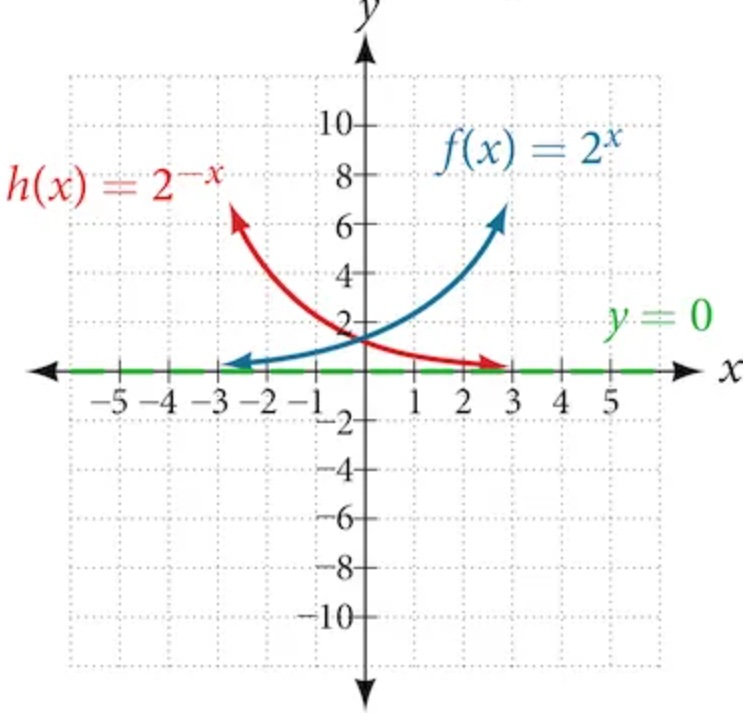
\includegraphics[width =2.8cm]{fig/exp2f.jpg}
\end{center}
\end{column}
\end{columns}

\end{frame}


\section{Trigonometry}



\begin{frame}\frametitle{Algebraic Functions}
\begin{columns}
\begin{column}{4.5cm}
An algebraic function provides a "y-value" for every "x-value"
\begin{itemize}
\item Linear: $y = x + 2$
\item Quadratic: $y = x^2$
\item Periodic: $y = sin(x)$
\end{itemize}
\end{column}
\begin{column}{7cm}
\begin{center}
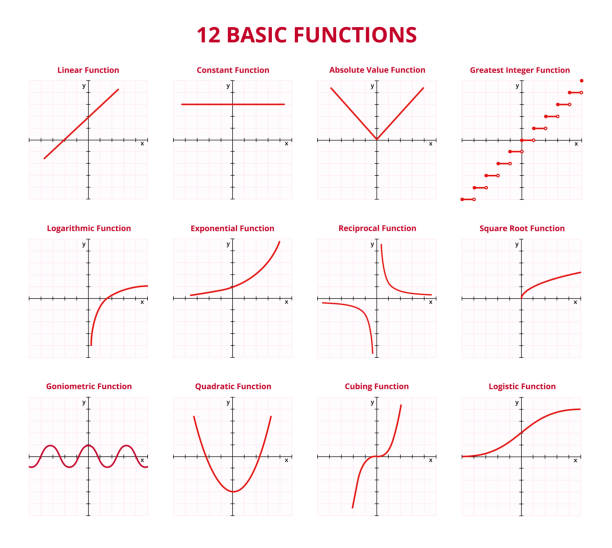
\includegraphics[width=7cm]{fig/basicfun.jpg}
\end{center}
\end{column}
\end{columns}
\end{frame}

\begin{frame}\frametitle{More Desmos Fun}

\begin{center}
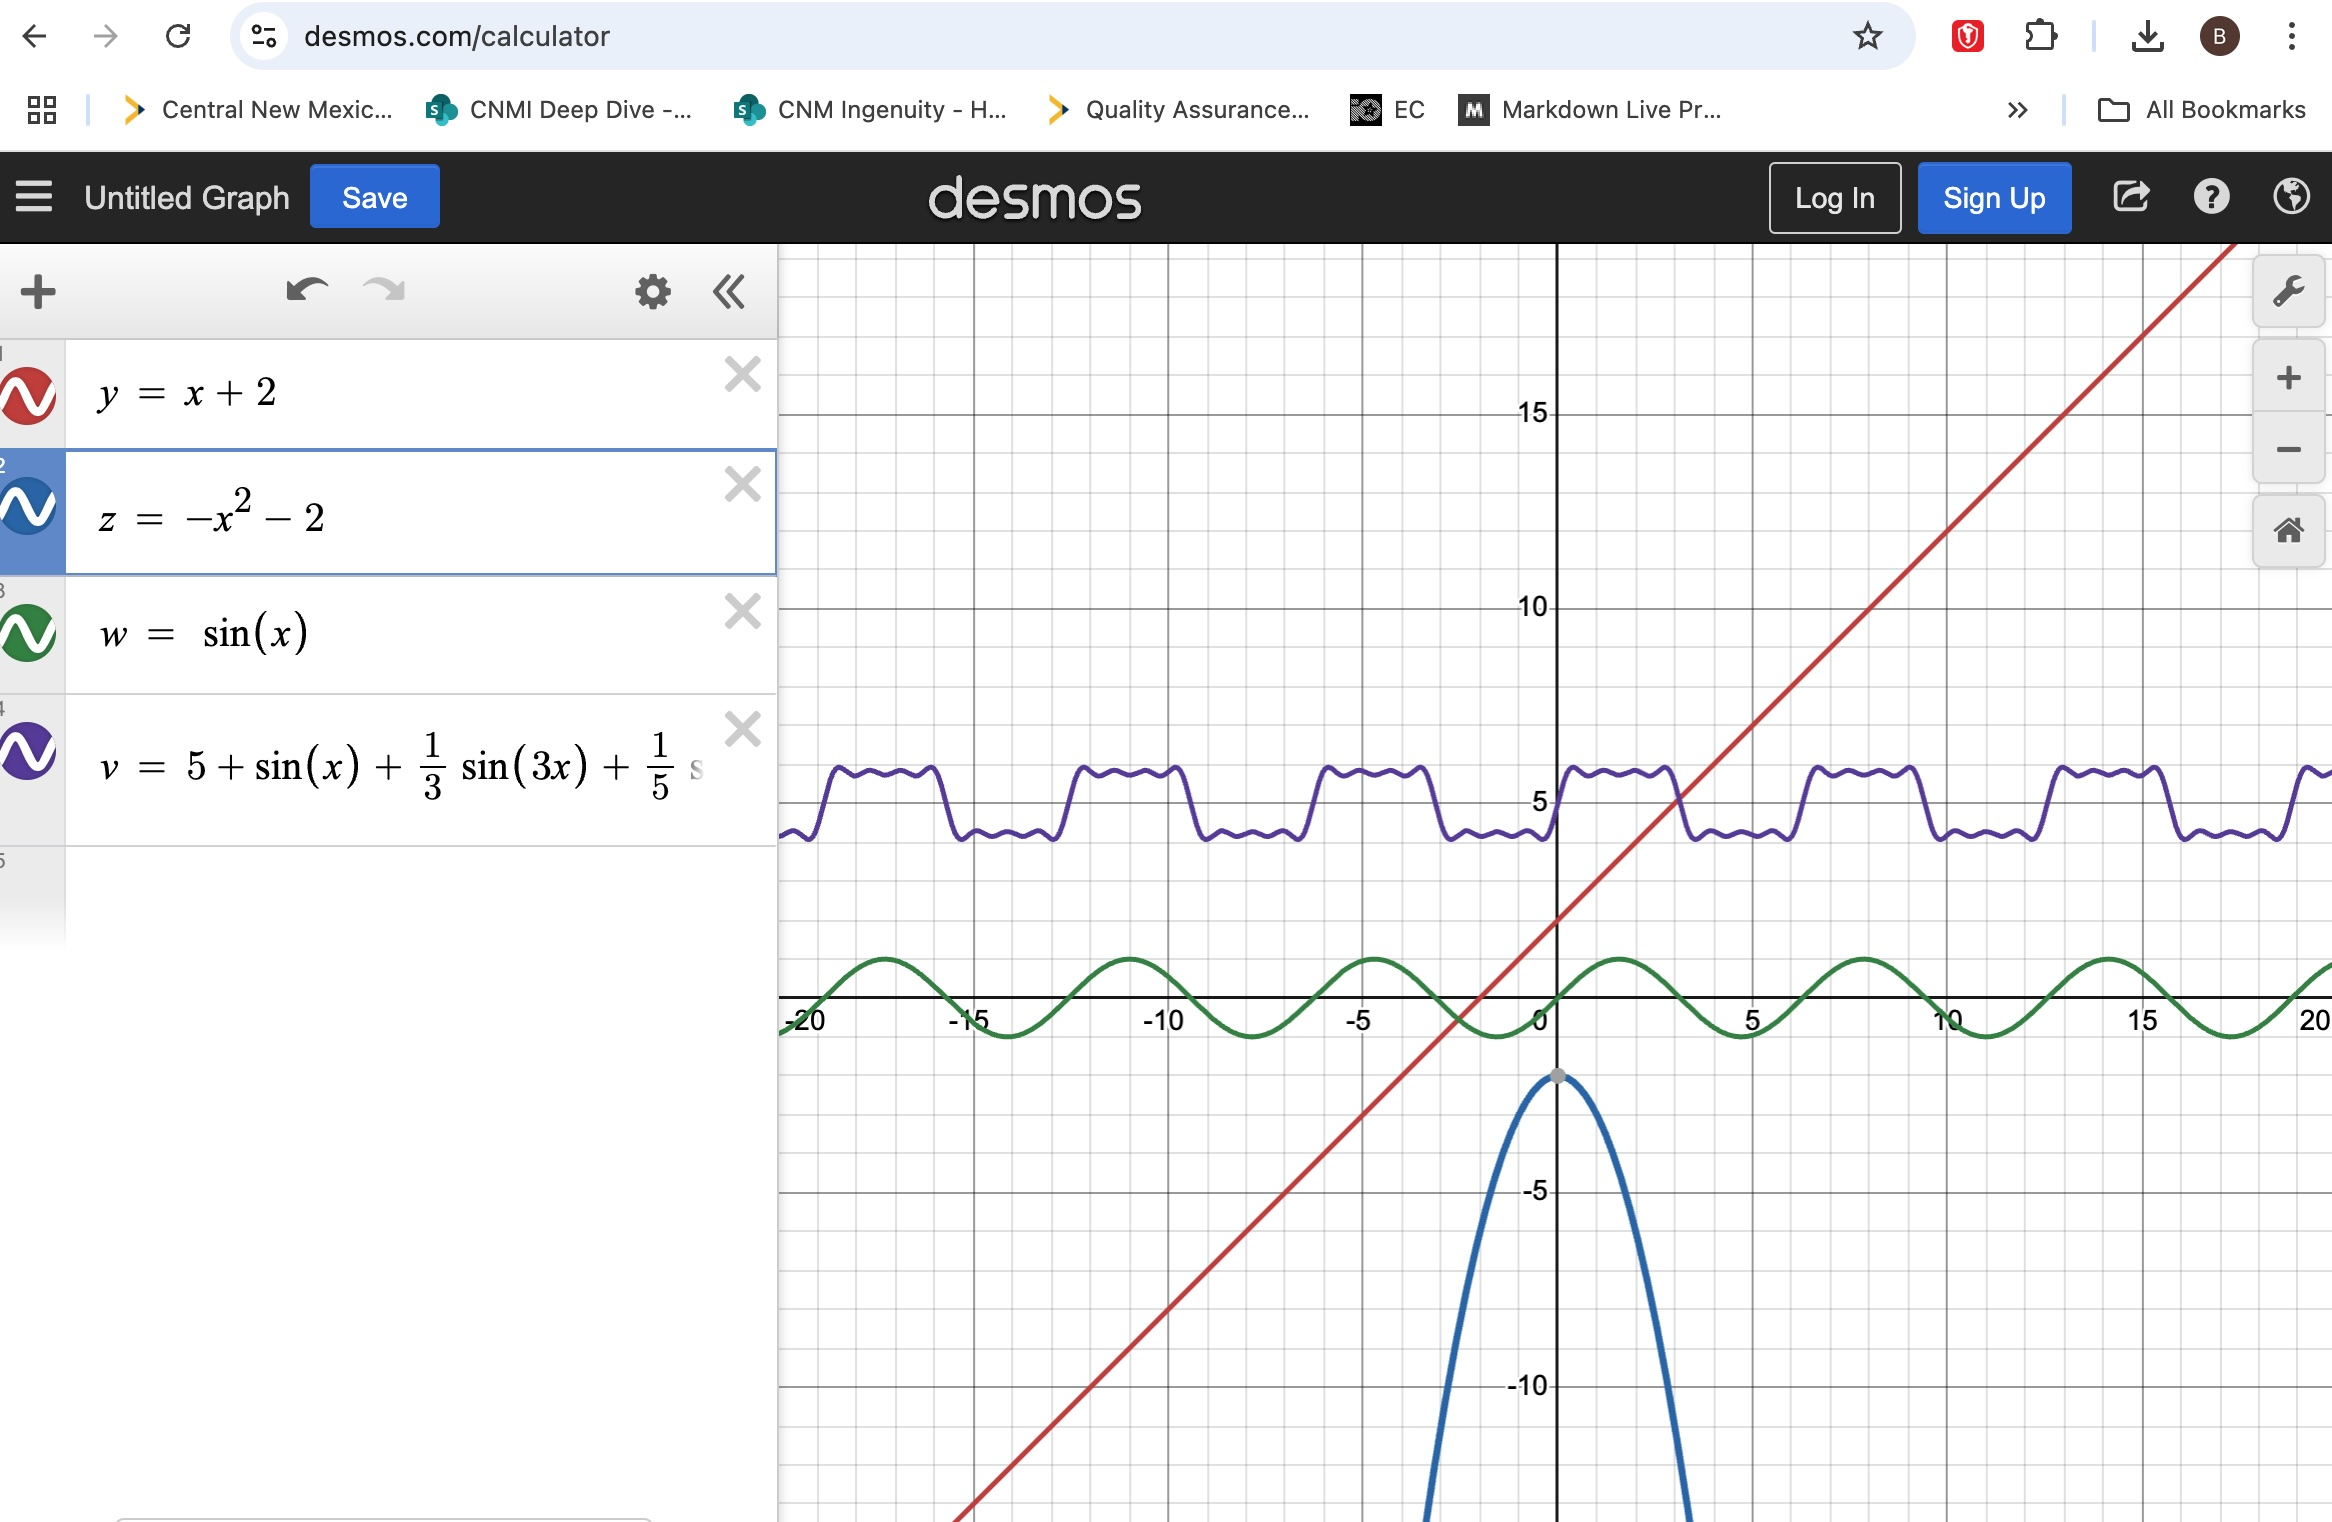
\includegraphics[width=12cm]{fig/desmosfun.jpg}
\end{center}
\end{frame}


\begin{frame}\frametitle{Pi ($\pi)$}

\begin{center}
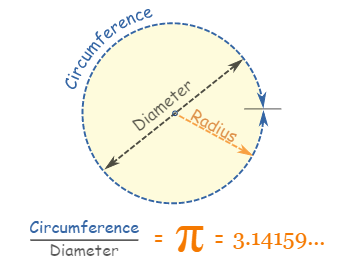
\includegraphics[width=8cm]{fig/pi.png}
\end{center}

\end{frame}


\begin{frame}\frametitle{Unit Circle and Trigonometric Functions}
The Unit Circle is a circle with a radius of 1.
\begin{columns}
\begin{column}{6cm}
\begin{center}
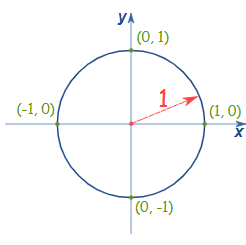
\includegraphics[scale=0.75]{fig/unitcircle.png}
\end{center}
\end{column}
\begin{column}{6cm}
\begin{center}
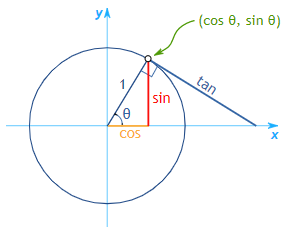
\includegraphics[scale=0.75]{fig/unitcircle_cst.png}
\end{center}
\end{column}
\end{columns}
The Unit Circle can be used to map out the trigonometric values of sine, cosine, and tangent.
\end{frame}


\begin{frame}\frametitle{Unit Circle and the Value of $sin(\theta)$}
\begin{columns}
\begin{column}{6cm}
\begin{center}
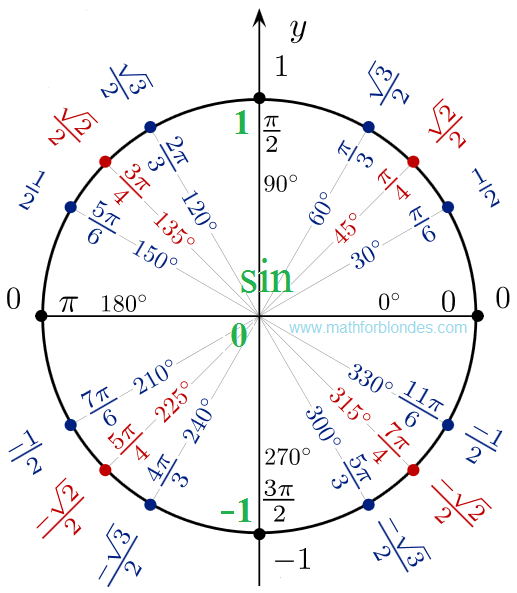
\includegraphics[scale=0.25]{fig/unitcircle_sin.png}
\end{center}
\end{column}
\begin{column}{6cm}
\begin{center}
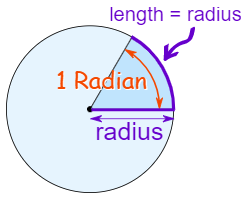
\includegraphics[scale=0.75]{fig/unitcircle_rad.png}
\end{center}
\end{column}
\end{columns}

\vspace{0.25cm}

\begin{itemize}
\item $sin(\theta)$ is the y-value of the point on the Unit Circle at angle $\theta$. 
\item In our trig functions, $\theta$ is measured in radians (rad), not degrees.
\item 360 degrees = $2 \pi$ radians.
\end{itemize}
\end{frame}



\begin{frame}\frametitle{Sine Waves}
\begin{center}
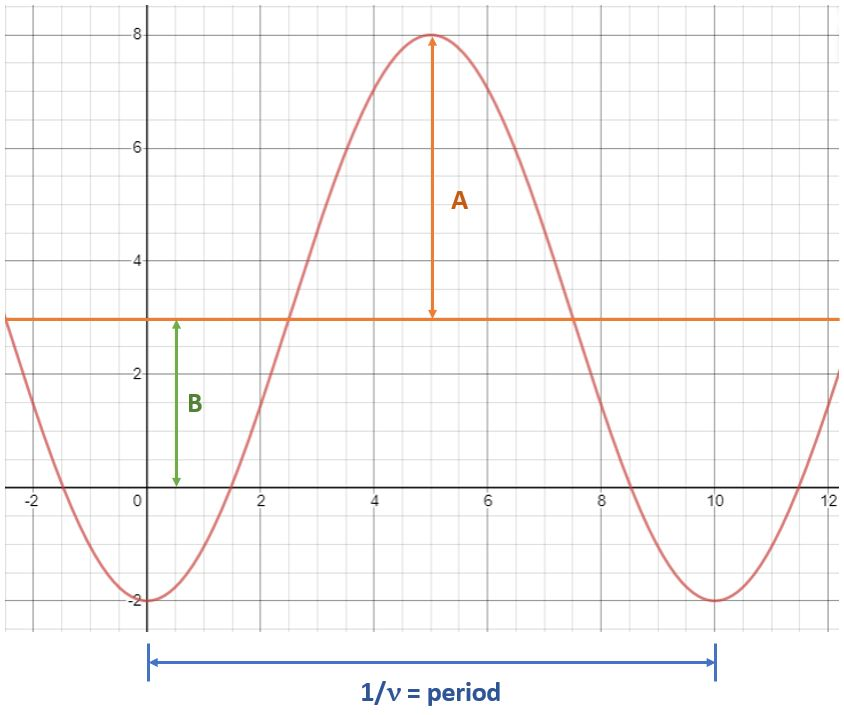
\includegraphics[scale=0.25]{fig/sin.jpg}
\end{center}

\begin{center}
$y = A * sin(2*\pi*\nu*t) + B$
\end{center}

where A = amplitude, B = offset, $\nu$ = frequency = $\frac{1}{period}$, 

and t = time in seconds.
\end{frame}


\begin{frame}\frametitle{Using Desmos (desmos.com/calculator)}
\begin{center}
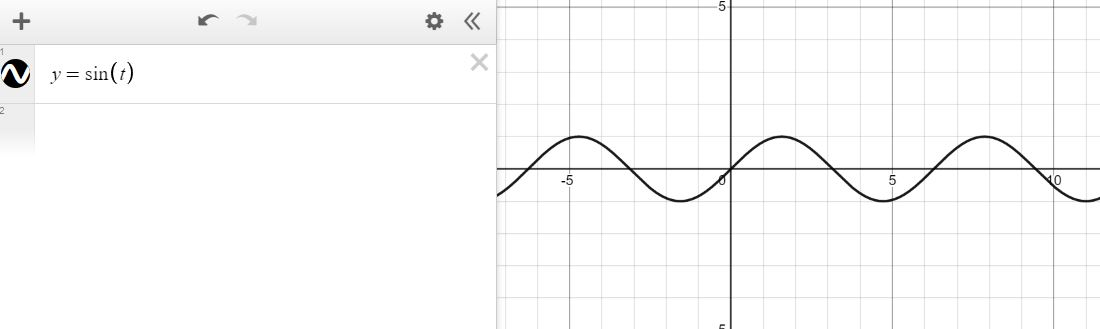
\includegraphics[scale=0.35]{fig/desmos1.jpg}
\end{center}
\begin{center}

\vspace{0.5cm}

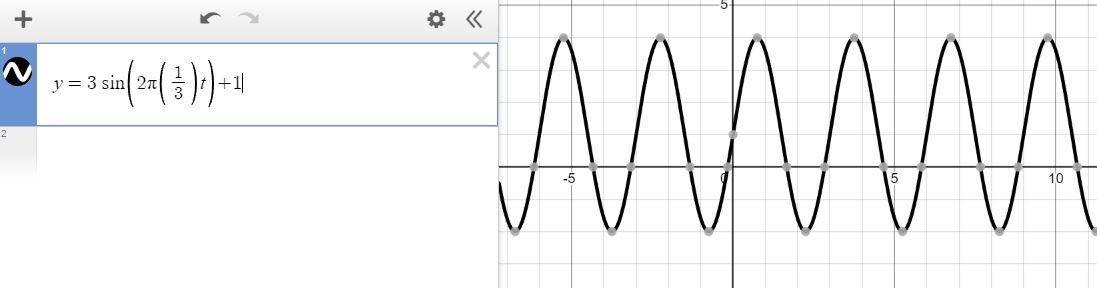
\includegraphics[scale=0.35]{fig/desmos2.jpg}
\end{center}
\end{frame}



\begin{frame}\frametitle{SOH CAH TOA}

\begin{itemize}
\item sin = opposite over hypotenuse
\item cos = adjacent over hypotenuse
\item tan = opposite over adjacent
\end{itemize}

\vspace{0.25cm}

\begin{center}
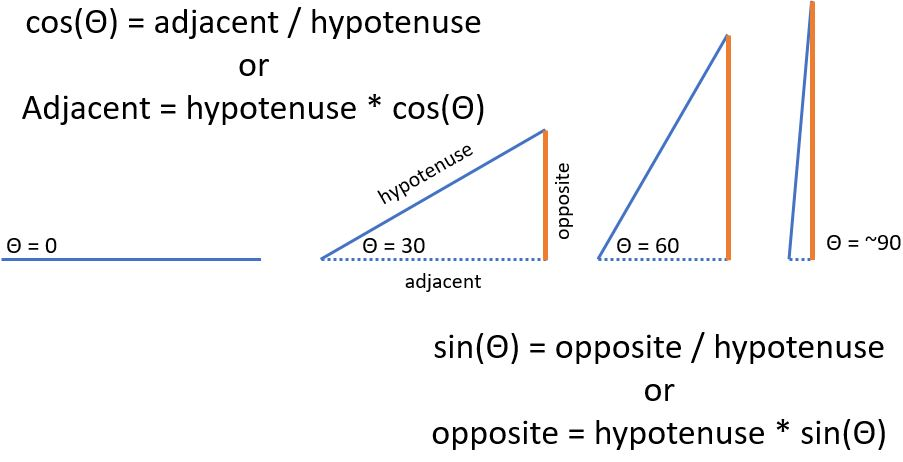
\includegraphics[scale=0.35]{fig/sohcahtoa.jpg}
\end{center}
\end{frame}

\section{Vectors}

\begin{frame}\frametitle{Scalars and Vectors}
Scalars are quantities that are fully described by a magnitude (or numerical value) alone.

Vectors are quantities that are fully described by both a magnitude and a direction.

\vspace{0.25cm}
\begin{center}
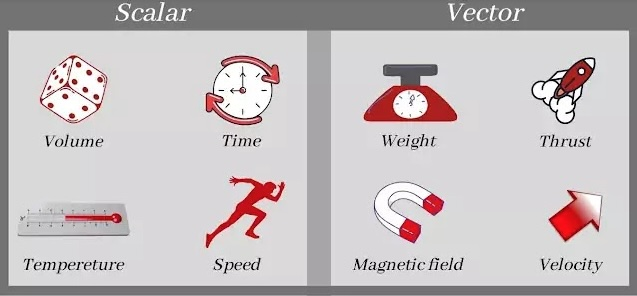
\includegraphics[width=8cm]{fig/scalarVector.jpg}
\end{center}
\end{frame}

\begin{frame}\frametitle{Pythagorean Theorem in 3 Dimensions}
\begin{columns}
\begin{column}{5cm}
\begin{center}
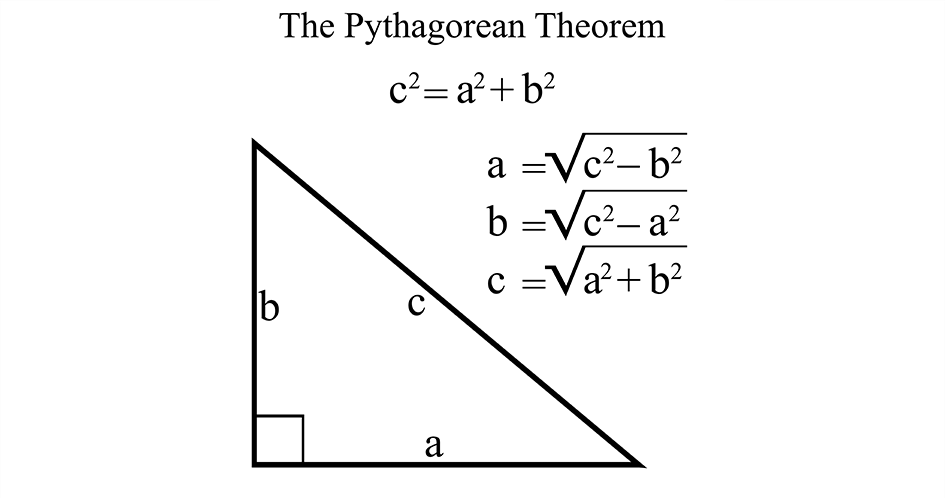
\includegraphics[width=5cm]{fig/pathagorean.png}

\vspace{0.25cm}

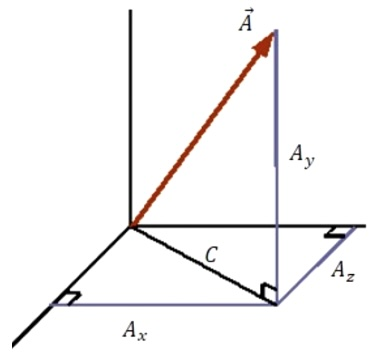
\includegraphics[width=4cm]{fig/pathag3D.jpg}

\end{center}
\end{column}
\begin{column}{5cm}
To add orthogonal (at right angles to each other) vectors in 3 Dimensions:
\begin{itemize}
\item $C = \sqrt{A_x^2 + A_y^2}$
\item $A_{total} = \sqrt{C^2 + A_z^2}$
\item $A_{total} = \sqrt{A_x^2 + A_y^2 + A_z^2}$
\end{itemize}
\end{column}
\end{columns}
\end{frame}



\end{document}
